\chapter{Knowledge-enabled Fault Tolerant Search}
\label{cha: search}

All the previous chapters have explained the process of knowledge generation from information gathered by the robot, in this chapter we would like to provide a motivating example of using this knowledge by the robot to make smart decisions. The problem we like to solve is to find people or objects in domestic environments, with the added information that the available vision detectors are faulty. Robots use sensors like camera, laser scanners, tactile sensors  to recognize objects and persons. While vision based object and person recognition is one of the most widely studied topics in artificial intelligence, even the best detectors still encounter failures. Most of the state-of-art detectors are based on machine learning methodologies. These detectors always publish their \emph{detection probability}. The detection probability quantifies the success rate of recognizing an object or person. This chapter explores methods of using our learned location probabilities and detection probabilities to accomplish a search task more efficiently in a domestic environment. 


Efficient searching for objects in the environment is one of the application for the knowledge being learned from object locations. The learned knowledge about location probabilities can be used as heuristics to improve the search time of objects. There are 2 basic methods in which we can use the learned knowledge as heuristics, first we can search for objects in the decreasing order of the learned probabilities or alternatively we can use the generative model to predict based on its learned probabilities. However the probabilistic representation of the learned knowledge can be used in ingenious way to solve more complex problems. 

\begin{figure}[htp]
\centering
\begin{subfigure}{.4\textwidth}
  \centering
  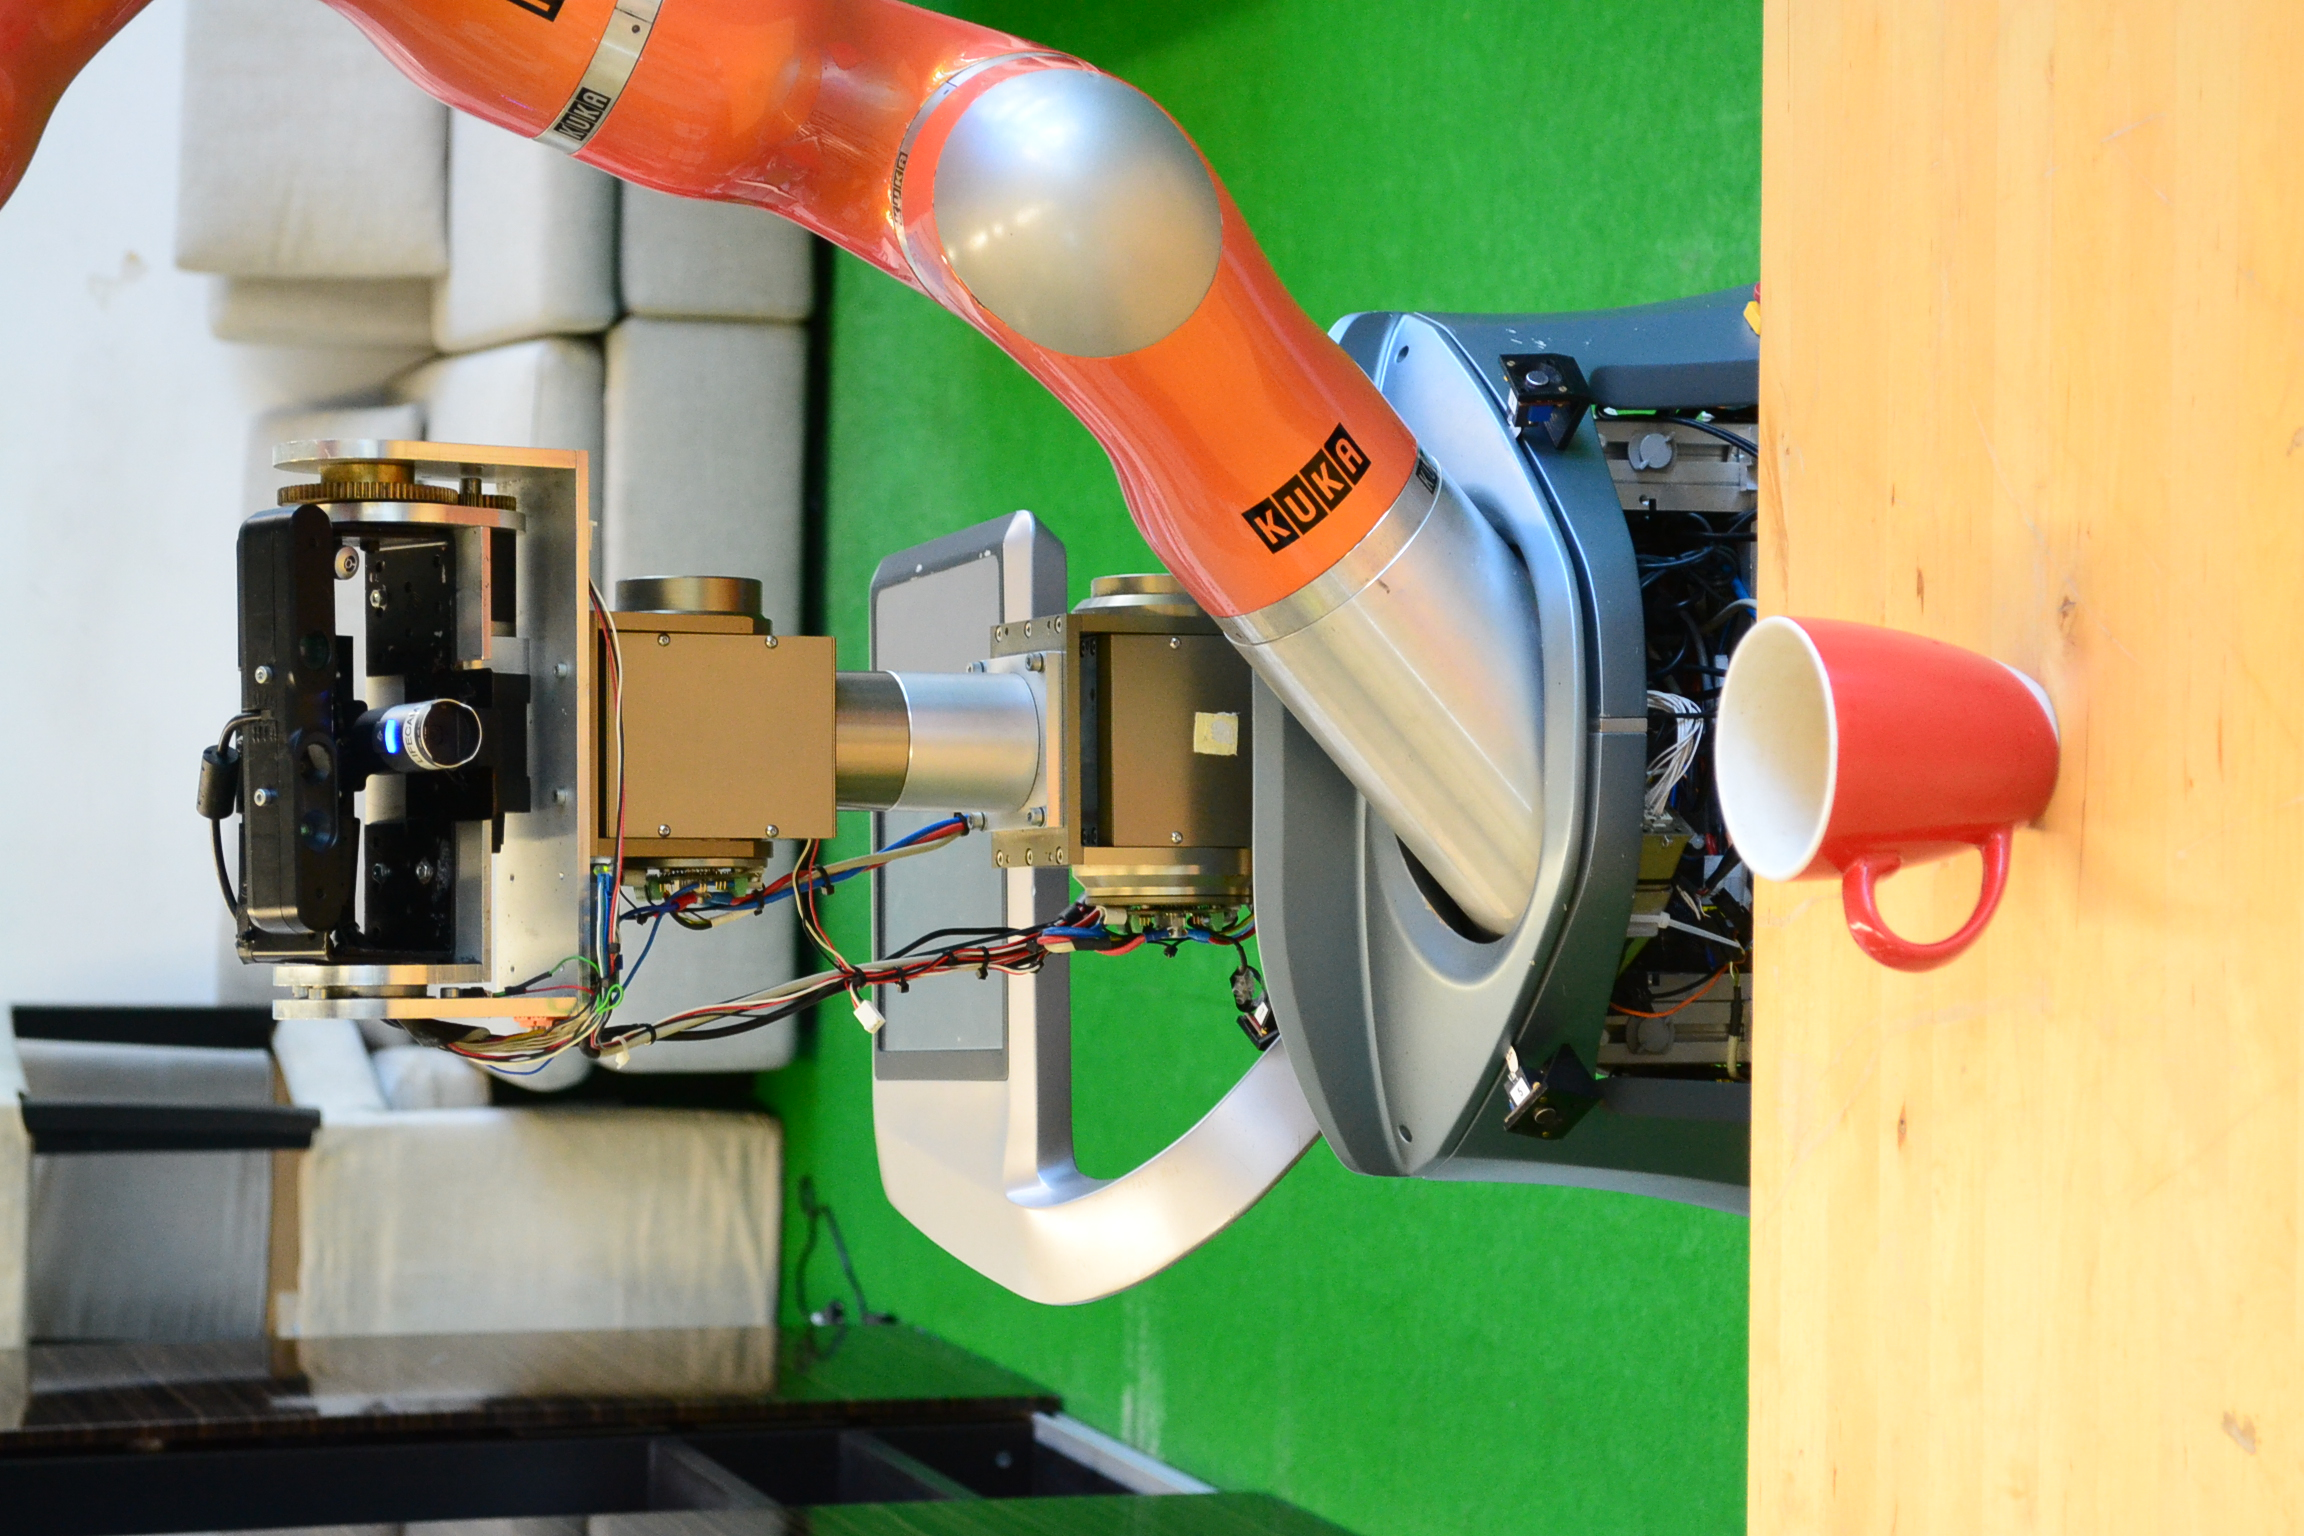
\includegraphics[width=0.9\linewidth, angle=-90]{images/robot_looking_cup.jpg}
\end{subfigure}%
\begin{subfigure}{.6\textwidth}
  \centering
  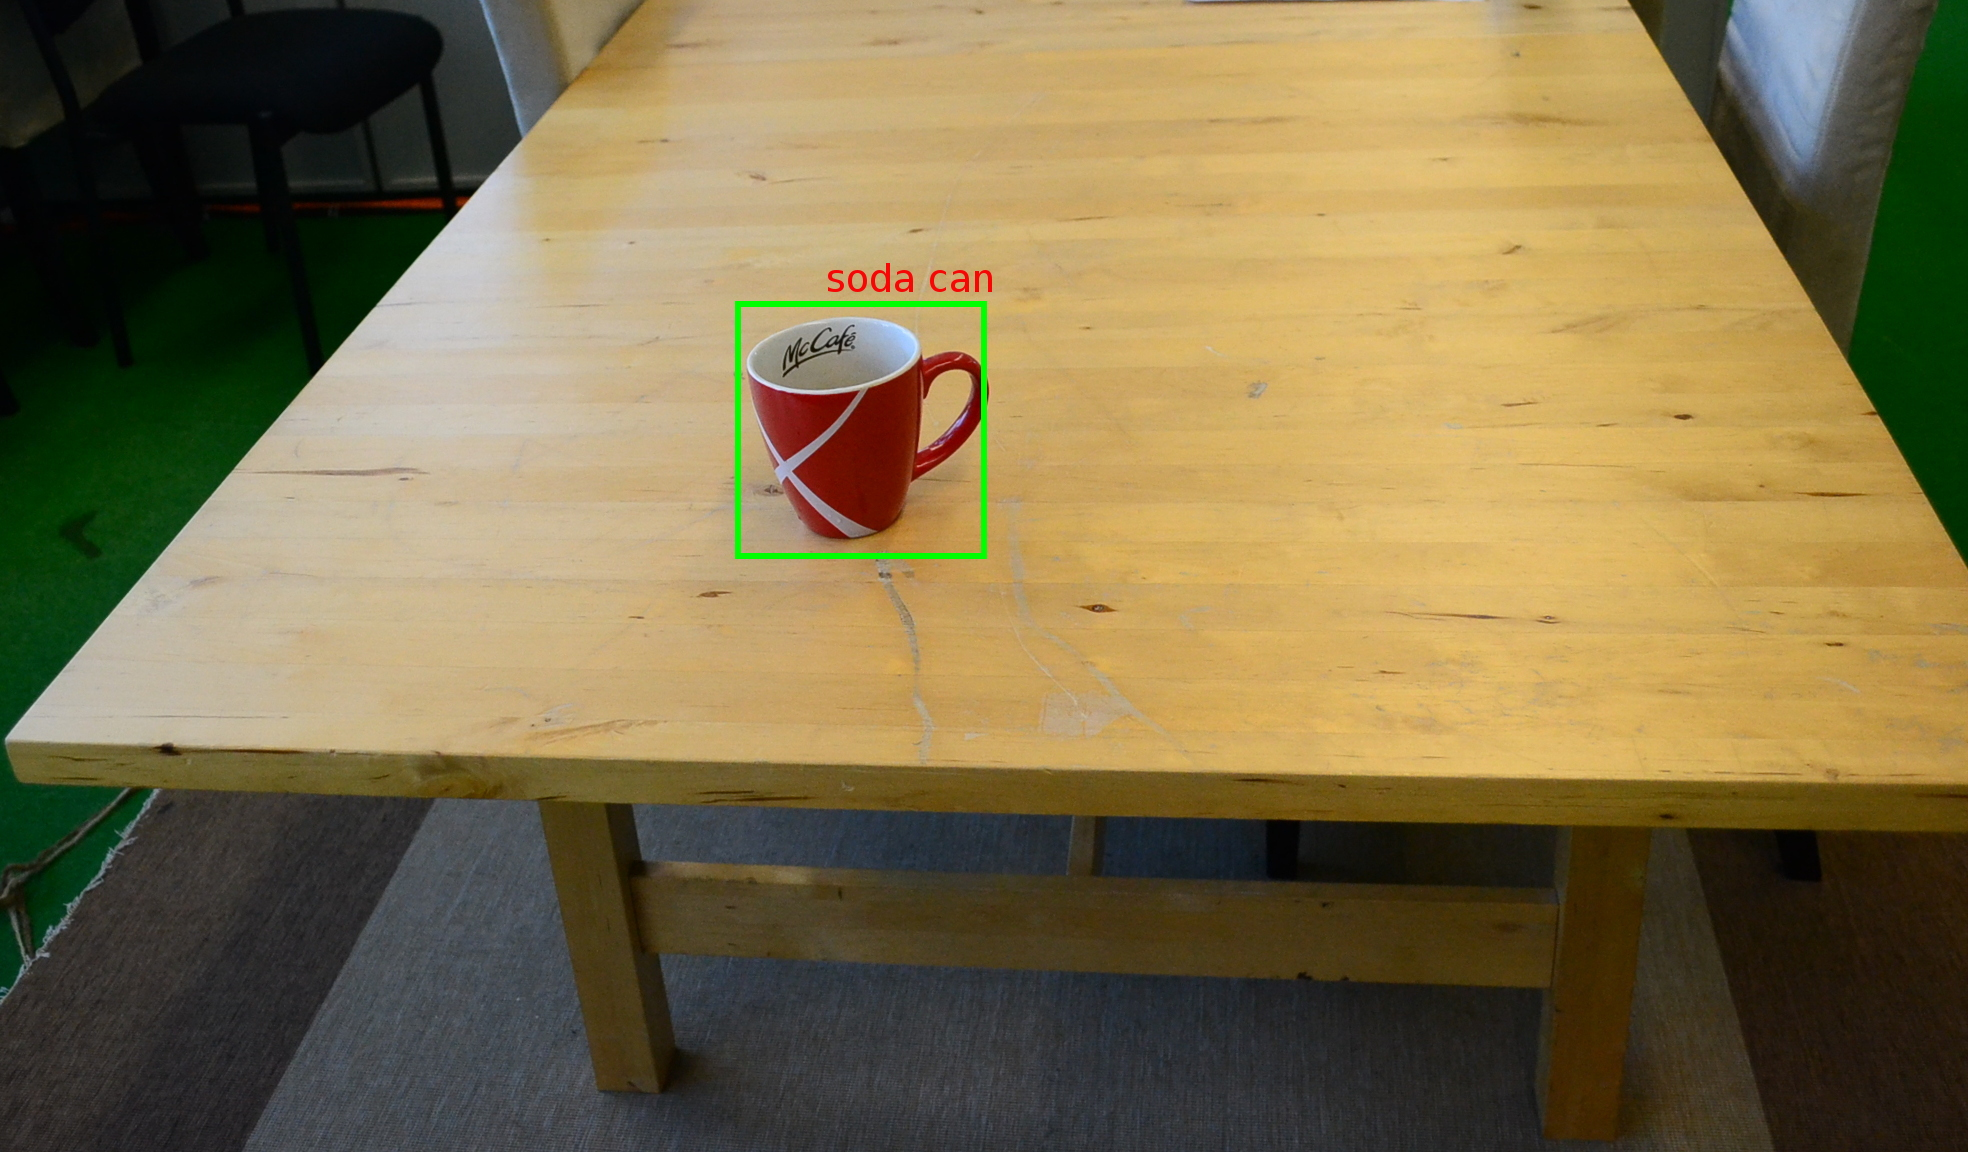
\includegraphics[width=\linewidth]{images/robot_view_cup.jpg}
\end{subfigure}
\caption[Fault tolerant search example]{Failures in object detection. The cup is misclassified as a soda can}
\end{figure}

In robotics \cite{chung2007decision} formulated the search control problem as a decision-making problem. This formulation of the search problem can include the information of false alarms and false detection. \cite{roy2003planning} demonstrated a system of finding people in a health care setting using a state probabilities of the people in a Partially Observable Markov Decision process planner. 

The above mentioned researchers have demonstrated how probabilities about locations can be used to make more informed decisions for the search problem. We here illustrate how the learned probabilities can be used to develop a \emph{sequential decision search algorithm} which can accommodate the recognition failure of the vision algorithms. The proposed algorithm here combines both the \emph{detection probability} and the \emph{learned probability} of the objects and provides sequential decisions for the next location to search.

\section{Probabilistic Search}

The robot is assumed to begin with map of the environment, learned knowledge as a probability distributions over where the people and objects might be located and the detection probability for each object and person. The robot can move around in the environment to look for the person or object, perceives the environment. 
The idea is to use the learned knowledge of the object locations as the first guess (prior ) of the probabilities that the object in question is located in each of the possible object locations \cite{cressie2015statistics}. The prior probabilities suggest which location to search first. If the object is not found in that location, the prior probabilities are then updated (yielding the posterior), and the process is repeated until the object is found. 

Assume that the domain of interest is a home we call $D_s$, which is made up of n spatial areas. Let $Y_i = 1$ if the object is in the \emph{i}th location, and then $Y_i = 0$ if it is not; $ i = 1, .... , n$. Now as discussed above object detectors can fail to detect the object. So, let $Z_i = 1$ if the object is found in the \emph{i}th location, and $Z_i = 0$ if not.

We can define two terms \emph{detection probability},
\begin{equation}
	p_i = Pr(Z_i = 1| Y_i =1), \qquad  i = 1,...,n,
\end{equation}
which is a conditional probability, and the \emph{occurrence probability},
\begin{equation}
	\pi_i = Pr(Y_i = 1),\qquad  i = 1, .... , n.
\end{equation}

This can be expressed in probabilistic programming form:
\begin{gather}
	Z_i | Y_i \sim Bernoulli (Y_i, p_i), \qquad  i  = 1,....,n \\
	Y_i \sim Bernoulli(\pi_i),\qquad   i = 1,...,n,
\end{gather}

where, the occurrence probability {$\pi_i$} is given by the learned probabilities, while the detection probability {$\pi_i$} is provided by the object detector algorithm.

Now, assume that hte \emph{i}th location is searched by the robot and the object is not found (i.e., $Z_i = 0$). In that case, the probability that the object is in the \emph{i}th location is updated using Bayes' Theorem. This yields the posterior probability,

\begin{gather*}
	Pr(Y_i = 1 | Z_i = 0) = \frac{Pr(Z_i = 0|Y_i=1)Pr(Y_i=1)} {Pr(Z_i=0)} \\
	                       = \frac{Pr(Z_i = 0| Y_i =1 )Pr(Y_i =1)}{Pr(Z_i=0|Y_i =1)Pr(Y_i = 1) + Pr(Z_i=0|Y_i=0)Pr(Y_i=0)} \\
	                       = \frac{(1 - p_i)\pi_i}{(1 - p_i)\pi_i + (1)(1 - \pi_i)} \\
	                       = \frac{(1 - p_i)\pi_i}{1 - p_i\pi_i}
\end{gather*}

where we assume that there are no false-positive detection (i.e., $Pr(Z_i =0| Y_i = 0) = 1$). Note that the new posterior is less than the prior probability $\pi_i$ as the object was not observed.

Since the object is not found in the searched location, then this should also affect the posterior probability in the other grid boxes. For example, consider the \emph{j}th location, where $j \neq i$. Then,
\begin{align*}
	Pr(Y_j = 1 | Z_i=0) &= \frac{Pr(Z_i = 0 | Y_j = 1)Pr(Y_j = 1)}{Pr(Z_i = 0)} \\
	                    &= \frac{\pi_j}{ 1 - p_i\pi_i}
\end{align*}

Thus, the posterior probability of the object being the \emph{j}th location is greater than the prior probability $\pi_j$ . These new posteriors will then become the next prior probabilities is a sequential procedure that would determine the next location to search.


\section{Example}

We illustrate a scenario and demonstrate how the robot performs its search based on two different search methodologies when there is fault caused by the object detector. The proposed probabilistic search is compared with a simple search method. Our aim is to find out the how by using probabilistic search the robot is making better search decisions in the presence of the fault.

We consider the scenario of a domestic robot in a home which is searching for an object. The robot has been in the home for long enough and made some observations. The robot has learned that the cup can be found 3 locations in the home, thus the domain for search can be defined as $D_s = \{cupboard, table, dishwasher \}$ . Based on these previous observations it also learns the occurrence probabilities as $p_i = \{ 0.8, 0.1, 0.1\}$ . Currently the cup is located in the cupboard \ref{fig:cup_in_cupboard} and the robot is asked to fetch the cup, so the robot searches the cupboard as its the most likely location based on prior beliefs. But the detector algorithm is not able to detect the cup and provides a faulty observation of the cup not found. 

We test the scenario using our proposed methods with 2 different detection probability

\begin{figure}[htp]
\centering
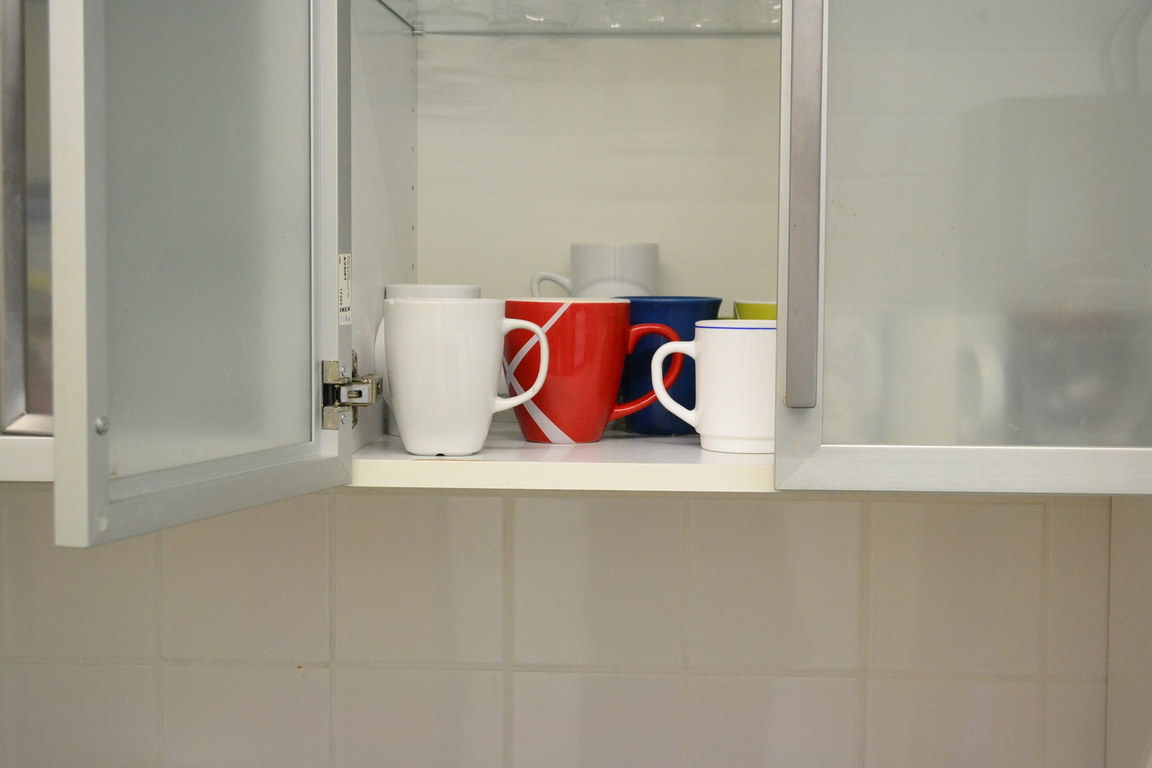
\includegraphics[width=0.4\textwidth]{images/cup_cupboard.jpg}
\caption[Probabilistic search example]{Example scenario of finding the cup which is located in the cupboard. The object detector is not able to recognize the object because of occlusion}
\label{fig:cup_in_cupboard}
\end{figure}

\begin{figure}[htp]
\centering
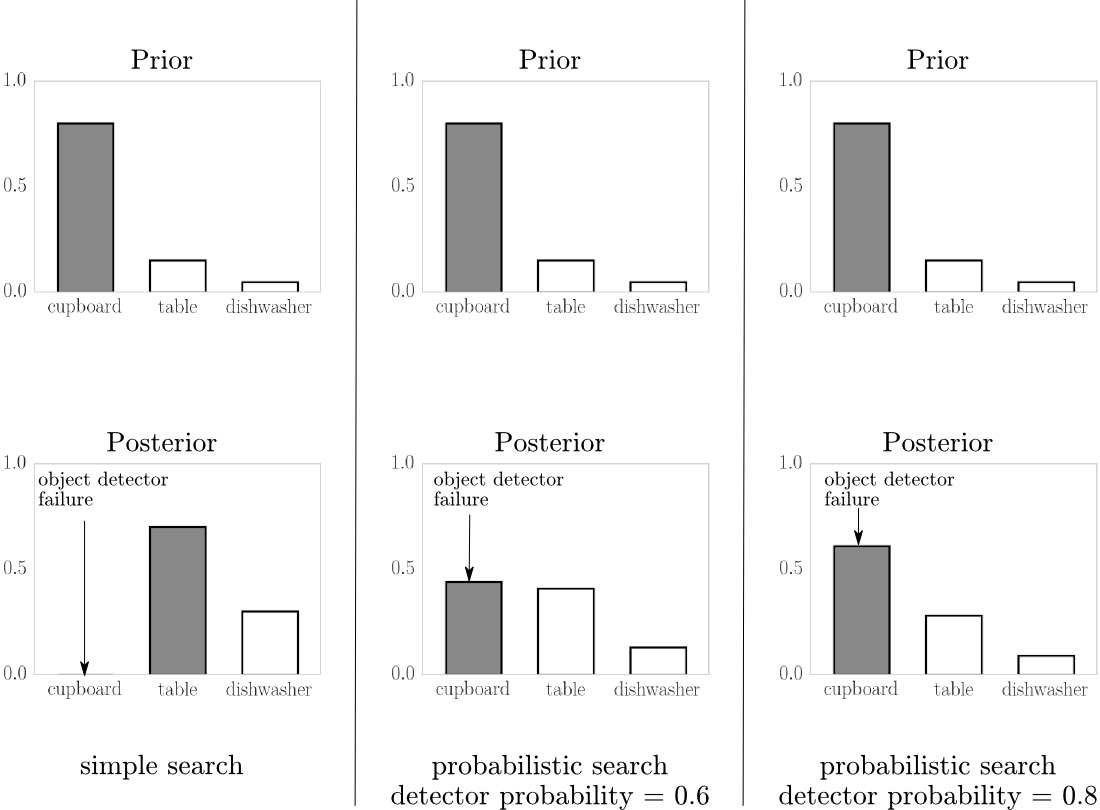
\includegraphics[width=\textwidth]{images/search.png}
\caption[Probabilistic search scenario]{The upper graphs shows the robots prior belief of the possible locations where the cup can be found. These beliefs at the outset have the probabilities which were previously learned by the robot. The shaded bar corresponds to the next location the robot will search. The lower-left graph shows the posterior probability(updated belief of the robot), when the detector fails to detect the object at the cupboard. Each column represents the change in belief based on the different search methods and detection probability. In probabilistic search the robot still has the belief that the cup is present in the cupboard while in simple search the robot will search the next location}

\label{fig:search_results}
\end{figure}

 
\subsection{Simple Search}

In simple search the robot goes to the highest probable location and on inability to find the object go to the next highest probable location. The search ends if the object is found or when the robot scans the least probable region. Thus in the above scenario the robot will first scan the cupboard if it finds the cup then it goes ahead and executes its task. If the robot fails to detect the cup in the cupboard it reduces the locations probability to $0$ and moves to next locations. Thus the default search sequence will be ${cupboard, table, dishwasher}$

\subsection{Probabilistic search}

Figure \ref{fig:search_results} illustrates probabilistic search algorithm. The heights of the bars in the graphs indicate the possibility of finding the object at the particular location. The upper graphs of Figure \ref{fig:search_results} shows that the prior beliefs of the robot which it had learned. As per the prior the robot is highly believes that the cupboard is the most likely place to search for the cup. The shaded bar in each graph represents the next location the robot will scan based on its current belief. So the robot goes ahead and scans the cupboard but the detector fails to detect the object. Now based on this new observation the robot goes ahead and re-allocates its belief. This re-allocated distribution is called the posterior distribution. The lower graphs in Figure \ref{fig:search_results} represents the posterior distribution after taking into account that the detector didn’t find the cup in the cupboard. Each column of the Figure \ref{fig:search_results} represents the different methods based on which the posteriors are updated. The first column is based on simple search which does not considers the detector probability. The middle column uses an object detector with 60\% detection probability, while the last column uses an object detector with 80\% detection probability. For the simple search the posterior has $0$ probability for the cupboard. Thus the robot has completely believed the object detector and considers that the object is not present in the cupboard, therefore as per the posterior the robot now moves to the next probable location. However, in probabilistic search the posteriors probability of cupboard is reduced , but not completely to $0$. As a result it still believes that the cup is present in the cupboard and tries again to search the cup in the cupboard. The reduction in the posterior probability of cupboard depends on the detector probability. 

This illustrates that the probabilistic search understands the limitation in the object detector and updates its beliefs to accommodate this limitation and make better \emph{informed} decisions.  


\section{Discussion}
In this chapter we proposed an approach that enables the robot combine the knowledge learned by robot about object location and the knowledge about the object detector, for making search decisions. Our approach uses Bayesian methods to incorporate the knowledge about the object detectors to make better search decisions. Furthermore with an illustrative example we showed how the robot makes knowledgeable decisions even when with false information from the object detector.
% chapter  (end)